\documentclass[letterpaper,9pt,journal]{IEEEtran}


\def\fourrr{seven }
\def\Fourrr{Seven }
%\documentclass[twocolumn,8pt]{extarticle}
\title{ \Huge Newtonian mechanics explained in \fourrr pages}
\author{Excerpt from the new book \href{http://minireference.com/}{\texttt{The NO BULLSHIT guide to MATH and PHYSICS}} by Ivan Savov} 


%\usepackage[papersize={5.5in,8.5in},verbose,bmargin=0.9cm,rmargin=0.7cm,lmargin=0.7cm,tmargin=0.9cm,headsep=0.3cm,footskip=0.5cm]{geometry}

\usepackage[letterpaper,bmargin=1.1cm,rmargin=0.95cm,lmargin=0.95cm,tmargin=1cm,headsep=0.2cm,footskip=0.5cm]{geometry}

\usepackage[english]{babel} %% Use your own babel language
\date{}


\usepackage{amsthm}
\usepackage{amsmath}
\usepackage{amssymb}
\usepackage{hyperref}

\def\mcal{\mathcal}
\def\eps{\epsilon}

\newcommand{\comment}[1]{\noindent [\textit{#1}]}



\usepackage{pdfpages}


\usepackage{textcomp}		% for 1/2



% Conditionally include sections using Hmin 
\usepackage{ifthen}
\newboolean{FORGINKO}
\setboolean{FORGINKO}{true}




\usepackage{wrapfig}



%\usepackage{standalone}

%\usepackage{enumitem}
%\setitemize{itemsep=-0.02in}   % LISTS WERE TOO AIRY



\newcommand{\settexitref}[2]{(\ref{#1}p\pageref{#1})}
\newcommand{\dokutitlelevelone}[1]{\chapter{#1}}
\newcommand{\dokutitleleveltwo}[1]{\section{#1}}
\newcommand{\dokutitleleveltree}[1]{\subsection{#1}}
\newcommand{\dokutitlelevelfour}[1]{\subsubsection{#1}}
\newcommand{\dokutitlelevelfive}[1]{\paragraph{#1}}
\newcommand{\dokufootnote}[1]{\footnote{#1}}
\newcommand{\dokufootmark}[1]{\footnotemark{#1}}
\newcommand{\dokubold}[1]{\textbf{#1}}
\newcommand{\dokuitalic}[1]{\textsl{#1}}
\newcommand{\dokumonospace}[1]{\texttt{#1}}
\newcommand{\dokuunderline}[1]{\underline{#1}}
\newcommand{\dokuoverline}[1]{\sout{#1}}
\newcommand{\dokusupscript}[1]{\textsuperscript{#1}}
\newcommand{\dokusubscript}[1]{$_{#1}$}
\newcommand{\dokuhline}{\line(1,0){400}}
\newcommand{\dokulabel}[1]{\label{#1}}
\newcommand{\dokuitem}{\item}
\newcommand{\dokuquoting}{\textbar}
\newcommand{\dokutabularwidth}{\textwidth}
% added by Ivan Savov
\newcommand{\dokuheadingstyle}[1]{#1}


\newcommand{\be}{\begin{equation}}
\newcommand{\ee}{\end{equation}}




\usepackage{tikz}
\usetikzlibrary{arrows,shapes,decorations,automata,backgrounds,petri}
\usetikzlibrary{shapes.gates.logic.US}
\usepackage[latin1]{inputenc}
% http://tex.stackexchange.com/questions/13933/drawing-mechanical-systems-in-latex/13952#13952
\usetikzlibrary{calc,patterns,decorations.pathmorphing,decorations.markings}





\begin{document}
\maketitle

%\vspace*{-1cm}

%

%\twocolumn[
%  \begin{@twocolumnfalse}
%\begin{center}
%\fontsize{27}{16}\selectfont
%%EZ \ MECHANICS \ TUTORIALS
%MECHANICS \ \  in \ \  FOUR PAGES
%\normalsize 
%%\vspace{2mm}
%%by Ivan Savov
%\vspace{6mm}
%\end{center}
%	%    \maketitle
%	%    \begin{abstract}
%	%      ...
%	%    \end{abstract}
%  \end{@twocolumnfalse}
%  ]
  

\begin{abstract}
%This document is a self contained tutorial on Mechanics.
Mechanics is the precise study of the motion of objects, the forces acting
on them and more abstract concepts such as momentum and energy.
You probably have an intuitive understanding of these concepts already,
but in the next \fourrr pages you will learn how to use precise mathematical
equations to support your intuition. All topics will be covered including prerequisites.
%This document is a complete course on
%Newtonian mechanics.
%Perhaps more importantly, we will also learn
%where the equations come from.
%There will be parties to go to and beers to drink later on in the semester, 
%so it is best to learn about all the important concepts of physics right now 
%and have time to chill later on in the semester. 
%%
%If you understand everything that is covered in the next \fourrr pages,
%I can guarantee you that you will be able to pass the final exam.
\end{abstract}



%
%\label{05f8e33b48d5f8430980e3d1f38e5116}%% mechanics

%Mechanics is the precise study of moving objects, forces and energy.
%You already have an intuitive understanding of these concepts,
%but in this chapter I will teach you how to use precise mathematical 
%models which will support your intuition.
%
%Mechanics is the part of physics that is most well understood.
%Ever since Newton figured out the whole $F=ma$ thing and 
%the law of gravitation, people have \emph{used} mechanics in order
%to achieve great technological feats. 

%There will be math, yes, but nothing too complicated.
%In fact, the hardest type of equation you will have to solve is a quadratic equation, so don't worry too much about that.
%The upshot of understanding the math, is that you will 
%be able to calculate and predict phenomena in the world around you
%simply by plugging numbers into the right equation.

\section*{Introduction}


%\section{Short Introduction}
%
To solve a physics problem is to obtain the \emph{equation of motion} $x(t)$, 
which describes position of the object as a function of time.
%
Once you know $x(t)$, you can answer many of the question pertaining to the motion of the object.
To find the initial position $x_i$ of the object, you simply plug $t=0$ into the equation of motion $x_i = x(0)$.
To find the time(s) when the object reaches a distance of 20[m] from the origin, we simply solve for $t$ in $x(t)=20$[m].
Many of the problems on you final exam in physics will be of this form, so it is really important that you know
how to find the equation of motion for any object.

%%\paragraph{{\bf Forces}}
The first step in finding $x(t)$ is to calculate all the \emph{forces} that act on the object.
Forces are the \emph{cause} of motion, so if you want to understand motion you need to understand forces. 
Newton's second law $\sum \vec{F} = \vec{F}_{net}=m\vec{a}$ states that forces acting on an object 
produce an \emph{acceleration} inversely proportional to the mass of the object. 
%Once you have the acceleration, you can compute $x(t)$ using two simple calculus steps.
%For now, though, we want to focus on the causes of motion: the forces acting on the object.
%There are many kinds of forces: the weight of an object $\vec{W}$ is a type force, 
%the force of friction $\vec{F}_f$ is another type another, the tension in a rope $\vec{T}$ yet another type of force
%and there are many others.
%Note the little arrow on top of each force, which is there to remind you that forces are \emph{vector} quantities.
%Unlike regular numbers, forces act in a particular direction, so it is possible that the effects of 
%one force are counteracting another force. For example the force of the weight of a flower pot 
%is exactly counter-acted by the tension in the rope on which it is suspended, thus,
%while there are two forces that may be acting on the pot, there is no \emph{net force} acting on it.
%Since there is no net force to cause motion and since the pot wasn't moving to begin with, 
%it will just sit there motionless despite the fact that there are forces acting on it!
%The first step when analyzing a physics problem will be calculation of 
%acting on the object, which 
The \emph{net force} on an object is the sum of all the forces acting on the object: 
$\vec{F}_{net} \equiv \sum \vec{F}$. Once you have $\vec{F}_{net}$ you know its 
acceleration using $\vec{a}=\frac{\vec{F}_{net}}{m}$.

It turns out that once you know the acceleration of an object $a(t)$, 
you can easily find its velocity $v(t)$ function and once you know the velocity 
function you can find the position function $x(t)$.
%The acceleration is the change in the velocity of the object, thus if you know
%that the object stated with an initial velocity of $v_i \equiv v(0)$,
%and you want to find the velocity at later time $t=\tau$, 
%you have to add up all the acceleration that the object felt during this time $v(\tau)=v_i+\int_0^\tau a(t)\;dt$.
\begin{equation}
 \frac{1}{m}\sum \vec{F} = a(t) \ \overset{v_i+ \int\!dt }{\longrightarrow} \ v(t) \ \overset{x_i+ \int\!dt }{\longrightarrow} \ x(t).
 \label{fma-eqn}
\end{equation}
The symbol $\int \cdot \;dt$ is called an \emph{integral} and is fancy way of finding the total
of some quantity over time. 

initial velocity of $v_i \equiv v(0)$,

initial position $x_i$

%The right hand side of the equation is called a \emph{dynamics} problem and involves 
%the calculation of the \emph{net force} $\vec{F}_{net} \equiv \sum \vec{F}$.
%The right hand side in the above equation is called \emph{kinematics} and focusses on
%the use of integration in order to find $v(t)$ from $a(t)$ and $x(t)$ from $v(t)$.
%Don't worry about this integration business; 
%it is quite simple and we will cover everything you need to know about it in the next section.  


%Newton's second law can also be applied to the study of circular motion.
%Circular motion is described by the angle of rotation $\theta(t)$, 
%the angular velocity $\omega(t)$ and the angular acceleration $\alpha(t)$.
%The causes of angular acceleration are angular force, which we call \emph{torques} $\mcal{T}$.
%Apart from this change to angular quantities, the principles behind the circular motion 
%are exactly the same as those for linear motion.
%and Newton's second law for rotational motion is $\mcal{T}_{net}=I\alpha$.
%We will 
%The quantity $I$ is called the \emph{moment of inertia} and describes how difficult it is to make an object turn.
%Circular motion is therefore 
%\begin{equation}
% \frac{1}{I}\sum \mathcal{T} = \alpha(t) \ \overset{\omega_i+ \int\!dt }{\longrightarrow} \ \omega(t) \ \overset{\theta_i+ \int\!dt }{\longrightarrow} \ \theta(t).
% \label{fma-eqn}
%\end{equation}


%\begin{equation}
%  U(h) = - \int_0^h  \vec{F}_g \cdot d\vec{y} = - \int_0^h  (- mg\hat{\jmath}) \cdot \hat{\jmath} \;dy    = mgh.
%  \nonumber
%\end{equation}

%
%During a collision between two objects there will be a sudden spike in the contact force between them,
%which can be difficult to measure and quantify.
%It is therefore not possible to use Newton's law $F=ma$ to predict the accelerations that occur during collisions.
%%and the resulting motion of the objects after they collide.
%In order to predict the motion of the objects after the collision we must use a \emph{momentum} calculation.
%An object of mass $m$ moving with velocity $\vec{v}$ has momentum $\vec{p}\equiv m\vec{v}$.
%The principle of conservation of momentum states that {\bf the total amount of momentum before and
%after the collision remains constant}. Thus, if two objects with initial momenta $\vec{p}_{i1}$ and $\vec{p}_{i2}$ collide,
%the total momentum before in the collision must be equal to the total momentum after the collision:
%\[
%	\sum \vec{p}_i = \sum \vec{p}_f 	
%	\qquad
%	\Rightarrow
%	\qquad
%	\vec{p}_{i1} + \vec{p}_{i2} 
%		=
%		\vec{p}_{f1} + \vec{p}_{f2}.
%\]
%Using this equation, it is possible to calculate the final momenta $\vec{p}_{f1}$, $\vec{p}_{f2}$
%of the objects after the collision. 

%
%Another way of solving physics problems is to use the concept of energy.
%Instead of trying to describe the entire motion of the object, 
%we can focus only on the initial parameters and the final parameters.
%The law of conservation of energy states that {\bf the total energy of the system is a constant}.
%Knowing the initial energy of a system, therefore, allows us to infer the final energy.


In the remainder of this document, 
we will learn more about each of the above concepts and ways of thinking. 
Before we begin with the physics material, we must introduce some mathematical
background, which will allow us to better understand the concepts.




%!TEX root = mechanics_miniref_flyer.tex

To solve a physics problem is to obtain the \emph{equation of motion} $x(t)$, 
which describes the position of the object as a function of time.
%
Once you know $x(t)$, you can answer any question pertaining to the motion of the object.
To find the initial position $x_i$ of the object, you simply plug $t=0$ into the equation of motion $x_i = x(0)$.
To find the time(s) when the object reaches a distance of 20[m] from the origin, you simply solve for $t$ in $x(t)=20$[m].
Many of the problems on the mechanics final exam will be of this form so,
if you know how to find $x(t)$, you will be in good shape to ace the exam.

%\paragraph{{\bf Forces}}
\vspace{-3mm}
\subsection{Dynamics is the study of forces}
The first step towards finding $x(t)$ is to calculate all the \emph{forces} that act on the object.
Forces are the \emph{cause} of motion, so if you want to understand motion you need to understand forces. 
Newton's second law $F=ma$ states that {\bf a force acting on an object produces an acceleration}
inversely proportional to the mass of the object. 
Once you have the acceleration, you can compute $x(t)$ using calculus.
We will discuss the calculus procedure for getting from $a(t)$ to $x(t)$ shortly.
For now, let us focus on the causes of motion: the forces acting on the object.
There are many kinds of forces: the weight of an object $\vec{W}$ is a type of force, 
the force of friction $\vec{F}_f$ is another type of force, the tension in a rope $\vec{T}$ is 
yet another type of force and there are many others.
Note the little arrow on top of each force, which is there to remind you that forces are \emph{vector quantities}.
Unlike regular numbers, forces act in a particular direction, so it is possible for the effects of 
one force to counteract the effects of another force. For example the weight of a flower pot 
is exactly counter-acted by the tension in the rope on which it is suspended, thus,
while there are two forces that are acting on the pot, there is no \emph{net force} acting on it.
Since there is no net force to cause motion and since the pot wasn't moving to begin with, 
it will just sit there motionless despite the fact that there are forces acting on it!
To find the \emph{net force} acting on the object you have to calculate 
the sum of all the forces acting on the object $\vec{F}_{net} \equiv \sum \vec{F}$.
Once you have the net force, you can use the formula $\vec{a}(t) = \frac{\vec{F}_{net}}{m}$ 
to find the acceleration of the object.

\vspace{-2mm}
\subsection{Kinematics is the study of motion}
If you know the acceleration of an object $a(t)$ as a function of time and its initial velocity $v_i=v(0)$, 
you can find its velocity $v(t)$ function at all later times. 
This is because the acceleration function $a(t)$ describes the change in the velocity of the object.
If you know that the object started with an initial velocity of $v_i \equiv v(0)$,
the velocity at a later time $t=\tau$ is equal to $v_i$ plus the ``total velocity change" between $t=0$ and $t=\tau$.
The mathematical way of saying this is $v(\tau)=v_i+\int_0^\tau a(t)\;dt$.
The symbol $\int \cdot \;dt$ is called an \emph{integral} and is a fancy way of finding the total
of some quantity over a given time period. 
To find the change in the velocity we calculate the total of $a(t)$ between $t=0$ and $t=\tau$.

To understand what is going on, it may be useful to draw an analogy with a scenario you are more familiar with.
Consider the function $\textrm{ba}(t)$ which represents your bank account balance at time $t$,
and the function $\textrm{tr}(t)$ which corresponds to the transactions (deposits and withdraws) on your account.
The function $\textrm{tr}(t)$ describes the change in the function $\textrm{ba}(t)$,
the same way the function $a(t)$ describes the change in $v(t)$.
Knowing the balance of your account at the beginning of the month,
you can calculate the balance at the end of the month as follows: $\textrm{ba}(30)=\textrm{ba}(0)+\int_0^{30} \textrm{tr}(t)\:dt$.

If you know the initial position $x_i$ and the velocity function $v(t)$ you can find the position function $x(t)$ by using integration again.  
We find the position at time $t=\tau$ by adding up all the velocity (changes in the position). 
The formula is $x(\tau) = x_i + \int_0^\tau v(t)\:dt$.


The entire procedure for predicting the motion of objects can be summarized as follows:
\begin{equation}
\frac{1}{m} \underbrace{ \left( \sum \vec{F} = \vec{F}_{net}  \right) }_{\text{dynamics}} = \underbrace{ a(t) \ \overset{v_i+ \int\!dt }{\longrightarrow} \ v(t) \ \overset{x_i+ \int\!dt }{\longrightarrow} \ x(t) }_{\text{kinematics}}.
 \label{fma-eqn}
\end{equation}
%
If you understand the above equation, then you understand mechanics.
My goal for the next couple of pages is to introduce you to all the concepts that 
appear in this equation and the relationships between them. 




\vspace{-3mm}
\subsection{Other stuff}

Apart from dynamics and kinematics, we'll discuss several other topics.
%which are part of a standard Mechanics class. 

Newton's second law can also be applied to the study of objects in rotation.
Angular motion is described by the angle of rotation $\theta(t)$, 
the angular velocity $\omega(t)$ and the angular acceleration $\alpha(t)$.
The causes of angular acceleration are angular forces, which we call \emph{torques} $\mathcal{T}$.
Apart from this change to angular quantities, the principles behind circular motion 
are exactly the same as those for linear motion.
%and Newton's second law for rotational motion is $\mcal{T}_{net}=I\alpha$.
%We will 
%The quantity $I$ is called the \emph{moment of inertia} and describes how difficult it is to make an object turn.
%Circular motion is therefore 
%\begin{equation}
% \frac{1}{I}\sum \mathcal{T} = \alpha(t) \ \overset{\omega_i+ \int\!dt }{\longrightarrow} \ \omega(t) \ \overset{\theta_i+ \int\!dt }{\longrightarrow} \ \theta(t).
% \label{fma-eqn}
%\end{equation}


%\begin{equation}
%  U(h) = - \int_0^h  \vec{F}_g \cdot d\vec{y} = - \int_0^h  (- mg\hat{\jmath}) \cdot \hat{\jmath} \;dy    = mgh.
%  \nonumber
%\end{equation}



During a collision between two objects, 
there will be a sudden spike in the contact force between them
which can be difficult to measure and quantify.
It is therefore not possible to use Newton's law $F=ma$ to predict the accelerations that occur during collisions.
%and the resulting motion of the objects after they collide.
In order to predict the motion of the objects after the collision we must use a \emph{momentum} calculation.
An object of mass $m$ moving with velocity $\vec{v}$ has momentum $\vec{p}\equiv m\vec{v}$.
The principle of conservation of momentum states that {\bf the total amount of momentum before and
after the collision is conserved}. Thus, if two objects with initial momenta $\vec{p}_{i1}$ and $\vec{p}_{i2}$ collide,
the total momentum before the collision must be equal to the total momentum after the collision:
\[
	\sum \vec{p}_i = \sum \vec{p}_f 	
	\qquad
	\Rightarrow
	\qquad
	\vec{p}_{i1} + \vec{p}_{i2} 
		=
		\vec{p}_{f1} + \vec{p}_{f2}.
\]
Using this equation, it is possible to calculate the final momenta $\vec{p}_{f1}$, $\vec{p}_{f2}$
of the objects after the collision. 


Another way of solving physics problems is to use the concept of energy.
Instead of trying to describe the entire motion of the object, 
we can focus only on the initial parameters and the final parameters.
The law of conservation of energy states that {\bf the total energy of the system is conserved}.
Knowing the total initial energy of a system allows us to find the final energy,
and from this calculate the final motion parameters.

We will discuss all of these topics in the remainder of the document.

\vspace{-1mm}
\subsection{The plan}

Most people think of mechanics as a horrible chore inflicted upon them
which requires complicated mathematical prerequisites.
Instead, I propose a different way of thinking about mechanics,
namely, as an opportunity to play {\sc lego} with a bunch of cool
scientific building blocks.
%

Of course, you must realize that simply reading this \fourrr page tutorial cannot 
make a Mechanics expert out of you.  
Mechanics expertise comes from solving exercises on your own.
What we \emph{can} do in \fourrr pages is go over all the important 
concepts and describe the physics formulas which connect these concepts.
The good news is that {\bf there are only twenty equations that you need to know
to understand mechanics}.
Don't worry about prerequisites.
The hardest math you will have to do is solving a quadratic equation
and we will cover everything you need to know about 
vectors and calculus in the next section.
Flip the page to continue.\hfill $\Rightarrow$

%\vspace{1cm}


\section{Preliminaries}

In order to understand the equations of physics you need to be familiar with
vector calculations and to know a bit about integrals. 
We will introduce these concepts in the next two subsections.

\vspace{-3mm}
\subsection{Vectors}

Forces, velocities, and accelerations are vector quantities.
A vector quantity $\vec{v}$ can be expressed in terms of its \emph{components}
or in terms of its \emph{length and direction}.
\begin{itemize}
%\item $\vec{v}=(v_x,v_y)$: A vector.
\item  $x$ axis:  The $x$ axis is the horizontal axis in the coordinate system.
\item  $y$ axis: The $y$ axis is \emph{perpendicular} to the $x$ axis.
\item  $v_x$: the \emph{component} of $\vec{v}$ along the $x$ axis.
\item  $v_y$: the \emph{component} of $\vec{v}$ along the $y$ axis.
\item  $\hat{\imath}\equiv(1,0),\hat{\jmath}\equiv(0,1)$: Unit vectors in the $x$ and $y$ directions. 
\item  $\|\vec{v}\|$: The length of the vector $\vec{v}$.
\item	 $\theta$: The angle that $\vec{v}$ makes with the $x$ axis.
%\end{itemize}
%Vectors are expressed with respect to a \emph{coordinate system}:
%\begin{itemize}
%Any vector can be written as $\vec{v}=v_x\hat{\imath}+v_y\hat{\jmath}$ or as $\vec{v}=(v_x,v_y)$.
\end{itemize}

Given the $xy$ coordinate system, we can denote a vector in three equivalent ways:
$
  \vec{v}  
  \ \equiv \ (v_x,v_y)
  \ \equiv \  v_x\hat{\imath} + v_y\hat{\jmath} 
  %\equiv v_x\hat{x} + v_y\hat{y} \equiv  (v_x,v_y)
  \ \equiv \ 
  \|\vec{v}\| \angle \theta
$.
%where $\|\vec{v}\|$ denotes the length of the vector $\vec{v}$ and
%$\theta$ is the angle that it makes with the $x$ axis.

Given a vector expressed as a length and direction $\|\vec{v}\| \angle \theta$,
we calculate its components using:
\[
  v_x = \|\vec{v}\| \cos\theta, \qquad \text{and} \qquad   v_y = \|\vec{v}\|\sin\theta.
\]
Alternately, a vector expressed in component notation $\vec{v}=(v_x,v_y)$ 
can be converted to the length-and-direction form as follows:
\[
 \|\vec{v}\|  = \sqrt{ v_x^2 + v_y^2 }, \qquad \text{and} \qquad \theta = \tan^{-1}\!\left( \frac{ v_{y} }{ v_{x} } \right).
\]
It is important that you know how to convert between these two forms;
the component notation is useful for calculations, 
whereas the length-and-direction form describes the geometry of vectors.


The \emph{dot product} between two vectors $\vec{v}$ and $\vec{w}$ 
can be  computed in two different ways:
\[
 \vec{v}\cdot\vec{w} = v_xw_x + v_yw_y = \|\vec{v}\| \|\vec{w}\| \cos\phi,
\]
where $\phi$ is the angle between the vectors $\vec{v}$ and $\vec{w}$.
The dot product calculates how similar the two vectors are.
For example, we have $\hat{\imath} \cdot \hat{\jmath} =0$
since the vectors $\hat{\imath}$ and $\hat{\jmath}$ are orthogonal --- they point in completely different directions.
%


%Calculus involves $f(t)$...

%You need calculus in order to do quantitative analysis of how variables
%change over time (derivatives) or sum up all kinds of contributions that
%add up to a total (integration).

%The basic quantities that will appear in the equations of physics are 
%measured in meters [m], seconds [s], meters per second [m/s],  meters per second squared [m/s$^2$] and
%Newtons [N]. You should always keep in mind which units are being used (meters vs. kilometres) and
%\emph{what type} the type quantity you are manipulating (length vs. velocity). 
%%
%You should also be aware whether the quantities are regular numbers 
%or \emph{vectors} with multiple components.


%\subsection{Derivatives}
%
%a

\vspace{-3mm}
\subsection{Integrals}
\label{3369022ed3e212789ba2790306add593}%% integrals
\begin{wrapfigure}{r}{0pt}
\includegraphics[width=100pt]{/Library/WebServer/Documents/miniref/data/media/calculus/integral_as_region_under_curve_t.png}
\end{wrapfigure}

An integral corresponds to the computation of an \emph{area}
under a curve $f(t)$ between two points:
\[
 A(a,b) \equiv \int_{t=a}^{t=b} f(t)\;dt.
\]
The symbol $\int$ is a mnemonic for \emph{sum}, 
since the area under the curve corresponds in some
sense to the sum of the values of the function $f(t)$
between $t=a$ and $t=b$.
The integral is the total amount of $f$ between $a$ and $b$.
%
%For certain functions, it is possible to find an anti-derivative function 
%$F(t)$ which is the ``running total'' of the total area under the curve. 
%The area under $f(t)$ between $a$ and $b$ is computed as the \emph{change} in $F(\tau)$:
%\[
% A(a,b) = F(b) - F(a).
%\]

%The anti-derivative function $F(\tau)$ is also known 
%as the \emph{indefinite integral} of $f(t)$ because it 
%corresponds to the integral calculation without the
%need to specify a \emph{definite} number for the upper limit:
%\[
% F(\tau) = \int^\tau_0 f(t)\;dt + F(0) = A(0,\tau) + F(0).
%\]
%We use the Greek letter $\tau$ (tau) to denote the input of $F$ since $t$
%is already used as the integration variable.

%The choice of $t=0$ as the starting point is 
%completely arbitrary.  We could have used a different
%starting point and obtained a different anti-derivative:
%\[
% F_2(\tau) = \int^\tau_{42} f(t)\;dt + F_2(42) = A(42,\tau) + F_2(42).
%\]
%Both $F$ and $F_2$ are anti-derivatives of the function $f$
%and contain all the information about the area under the curve
%\[
%  A(a,b) = F(b) - F(a) = F_2(b) - F_2(a).
%\]
%The effect of the choice of the starting point is to
%add or subtract a constant term to the anti-derivative.
%All anti-derivatives of the function $f(t)$ differ only by
%an additive constant factor $F=F_2 + C$.
%We call $C$ the integration constant, and its value
%is usually specified by external conditions.

\begin{wrapfigure}{r}{0pt}
\includegraphics[width=110pt]{/Library/WebServer/Documents/miniref/data/media/calculus/simple_integral_one_tikz-0.png}
\end{wrapfigure}

Consider for example the constant function $f(t)=3$.
Let us find the expression $F(\tau)\equiv A(0,\tau)$
that corresponds to the area under $f(t)$ between 
$t=0$ and the time $t=\tau$.
We can easily find this area because the region under the curve is rectangular:
\[ 
 \! F(\tau) \equiv A(0,\tau) =  \! \int_0^\tau \!\! f(t)\;dt  = 3 \tau
\]
since the area of a rectangle is equal to the length of the base times the height.


\begin{wrapfigure}{r}{0pt}
\includegraphics[width=110pt]{/Library/WebServer/Documents/miniref/data/media/calculus/simple_integral_two_tikz-0.png}
\end{wrapfigure}

Anther important calculation is the area under 
the function $g(t)=t$. We will compute $G(\tau)\equiv A(0,\tau)$,
which corresponds to the area under $g(t)$ between $0$ and $\tau$.
This area is also easily computed since the region under the curve 
is triangular:
\[
 G(\tau) \!\equiv \!A(0,\tau) \!=\!\! \int_0^\tau \!\!\!g(t) \: dt \!= \!\frac{\tau\times\tau}{2} \!= \!\frac{1}{2}\tau^2
\]
since the area of a triangle is the product of the length of
the base times the height divided by two.


%We were able to compute the above integrals thanks to the
%simple geometry of the areas under the curves. Later on in
%this book we will develop techniques for finding 
%integrals of more complicated functions.
%
%In fact, there is an entire course, Calculus II,
%which is dedicated to the task of finding integrals.

For the purpose of understanding mechanics,
what you need to know is that the integral of a function is the total amount of the function accumulated during some time period. 
You should also try to remember the formulas:
\[
 \int_c^\tau a \;dt = a\tau + C, \qquad 
 \int_c^\tau at \;dt = \frac{1}{2}a\tau^2 + C,
\]
which correspond to the integral of a constant function
and the integral of a line with slope $a$.
%Note how we always add an additive constant term $+C$ when
%we state integral formulas. This is to remind  us that the 
%answer has an extra parameter (an additive constant term),
%which must be specified by the problem.
Note that each time you give a general integral formula
the answer will contain an additive constant term $+C$,
which depends on the starting point of the area calculation. 
In the above examples we used $c=0$ as the initial
point so we had $C=0$.

The integral of the sum of two functions is the sum of their integrals.
Using this fact and the two formulas above, 
we can also compute the integral for the function $f(t)=mt+b$ as follows:
\be
% F(\tau)=
%  \int_0^\tau f(t)\;dt =
  \int_c^\tau (mt + b)\;dt 
%  =  \int_0^\tau \!mt\;dt\  + \int_0^\tau \!b\;dt
 = \frac{1}{2}m\tau^2 + b \tau  + C.
  \label{integral-formula}
\ee


Now that you know about vectors and integrals, 
we can start our discussion of the laws of physics.


\section{Kinematics}
\label{sec:kinematics}

Kinematics (from the Greek word \emph{kinema} for \emph{motion}) is the study of the
trajectories of moving objects.  
The equations of kinematics can be used to calculate how long a ball thrown upwards will stay in the air, 
or to calculate the acceleration needed to go from 0 to 100 km/h in 5 seconds.

\vspace{-3mm}
\subsection{Concepts}
\label{408d82ccb63ca28fa1665f5ee146b453}%% position_velocity_and_acceleration_revisited

The key notions used to describe the motion of an objects are:
\begin{itemize}
\item  $t$: the time, measured in seconds [s].
\item  $x(t)$: the position of an object as a function of time --- also known as the equation of motion. % Measured in meters [m].
\item  $v(t)$: the velocity of the object as a function of time.% [m/s]
\item  $a(t)$: the acceleration of the object as a function of time. %[m/s$^2$]
\item  $x_i=x(0), v_i=v(0)$: initial position and velocity (initial conditions).
\end{itemize}

The position, velocity and acceleration functions ($x(t)$, $v(t)$ and $a(t)$) are connected. 
They all describe different aspects of the same motion.
The function $x(t)$ is the main function since it describes the position of the object at all times.
The velocity function describes the change in the position over time, hence it is measured in [m/s].
The acceleration function describes how the velocity changes over time.
%A constant positive acceleration means the velocity of the motion 
%is steadily increasing, like when you press the gas pedal in your car.
%A constant negative acceleration means the velocity is steadily decreasing,
%like when pressing the brake pedal.
%{\bf If you know the exact function $x(t)$}, then you can compute its \emph{derivative}
%and obtain the velocity function $v(t)$. You can obtain the acceleration function $a(t)$
%by computing the derivative of the velocity $v(t)$:
%\[
%  a(t) \overset{\frac{d}{dt} }{\longleftarrow} v(t) \overset{\frac{d}{dt} }{\longleftarrow} x(t).
%\]

Assume now that we know the acceleration of the object $a(t)$ and that we want to find $v(t)$.
The acceleration is the change in the velocity of the object, 
thus if you know that the object started with an initial velocity of $v_i \equiv v(0)$,
and you want to find the velocity at later time $t=\tau$, 
you have to add up all the acceleration that the object felt 
during this time $v(\tau)=v_i+\int_0^\tau a(t)\;dt$.
The velocity as a function of time is given by the initial 
velocity $v_i$ plus the integral of the acceleration.

If we integrate the velocity function, 
we will  obtain the position function $x(t)$.
Thus, the procedure for finding $x(t)$ starting from $a(t)$ can be summarized as follows:
\[
 a(t) \ \ \overset{v_i + \int\!dt}{\longrightarrow} \ \ v(t) \ \  \overset{x_i+ \int\!dt }{\longrightarrow} \ \ x(t).
\]

We will now illustrate how to apply this procedure for the important special 
case of motion with constant acceleration.

\vspace{-3mm}
\subsection{Uniform acceleration motion}

Suppose that an object starts from an initial position $x_i$ with initial velocity $v_i$ and 
undergoes a constant acceleration $a(t)=a$ from time $t=0$ until $t=\tau$.
What will be its velocity $v(\tau)$ and position $x(\tau)$ at time $t=\tau$?
 
%This is how the \emph{equations of motion} are derived. 
%Assuming that the acceleration is constant in time $a(t) =a$,
We can find the velocity of the object %at any time $t=\tau$ 
by integrating the acceleration from $t=0$ until $t=\tau$:
%\emph{adding up} all the acceleration from $t=0$ (integrating)
%to obtain the change in the velocity
\begin{align*}
 v(\tau) = v_i + \int_0^\tau a(t) \ dt &= v_i + \int_0^\tau a \ dt = v_i + a\tau,
\end{align*}
where we used the formula for the integral of a constant function. To obtain $x(t)$ we integrate $v(t)$ and obtain:
\begin{align*}
 x(\tau) = x_i + \int_0^\tau v(t) \; dt &= x_i + \int_0^\tau (at+v_i) \; dt = x_i + \frac{1}{2}a\tau^2 + v_i\tau,
\end{align*}
where we used the integral formula from equation \eqref{integral-formula}.
Note that the above integral calculations required the knowledge of the initial conditions $x_i$ and $v_i$.
This is because the integral calculations tell us the \emph{change} in the quantities relative to their initial values.
%so we must add
%the initial conditions 
%in the velocity $\int_0^\tau a(t)\;dt %= \Delta v 
%= v(\tau)-v_i$. 
%so must add $v_i$ to obtain $v(t)$.
%Similarly, the calculation of $x(\tau)$ required us to know the initial position $x_i$. 

% the above calculations required involved using the initial  calculation of $v(t)$ both integrals 
%so in order to find $v  from
%$t=0$ until $t=\tau$: and we have to add the finding the exact velocity function $v(t)$ required the knowledge of
%the initial velocity $v_i=v(0)$. Indeed, 




%\subsubsection{Formulas}

We can summarize our findings regarding uniform acceleration motion (UAM)
in the following three equations: 
\begin{align}
  a(t) &= a, \qquad \qquad \qquad \qquad  \text{(by the definition of UAM)} \nonumber \\
  v(t) &= at + v_i, 				  \label{UAM-v} \\
  x(t) &= \tfrac{1}{2}at^2 +  v_i t + x_i. \label{UAM-x}
\end{align}
These equations fully describe all aspects of the motion of an object undergoing a 
constant acceleration $a(t)=a$ starting from $x(0)=x_i$ with initial velocity $v(0)=v_i$.
%
There is also another very useful formula to remember:
%\[
% v(t)^2 = v_i^2 + 2a[x(t)- x_i],
%\]
%which is usually written
\be
 v_f^2 = v_i^2 + 2a(x_f-x_i), %\Delta x,
\ee
which is obtained by combining equation \eqref{UAM-v} and \eqref{UAM-x} in a particular way.

A special case of the above equations is the case with zero acceleration $a(t)=0$.
If there is no acceleration (change in velocity) then the velocity of the motion will be
constant so we call this \emph{uniform velocity motion} (UVM). 
The equations of motion for UVM are $v(t)=v_i$ and $x(t)=v_it + x_i$.
If you understand the difference between UVM and UAM and the three formulas above,
then you are ready to solve \emph{any} kinematics problem. % which you will run into.

\vspace{-3mm}
\subsection{Free fall}

We say that an object is in \emph{free fall} if the only force acting on it is the force of gravity.
On the surface of the earth, the force of gravity will produce a constant acceleration
of $a=-9.81$[m/s$^2$]. The negative sign is there because the gravitational acceleration
is directed downwards, and we assume that the $y$ axis points upwards.
% measure distance from the ground up.
% towards the center of the Earth.

\medskip
%That is it. Chapter done. 
You can test your knowledge by trying the following practice problems.


%{\bf Moroccan example.}
%Your friend drops a ball wrapped in aluminum foil from a 
%balcony located at a height of $x_i=44.145$[m] at $t=0$[s], 
%and it hits the ground at exactly $t=3$[s].
%What was the acceleration of the ball during its flight? 
%\ \ \ Ans: $a=\frac{-2 \times 44.145}{9}=-9.81$[m/s\^{ }2] (a.k.a. free fall).

{\bf 0 to 100 in 5 seconds.}
You want to go from $0$ to $100$[km/h] in $5$ seconds with your car.
How much acceleration does your engine need to produce?
Assume the acceleration is constant. \ Sol: Use \eqref{UAM-v}. Ans: $a=5.56$[m/s$^2$].



{\bf Moroccan example.}
Suppose your friend wants to send you a ball wrapped in aluminum 
foil from his balcony, which is located at a height of $x_i=44.145$[m]. 
At  $t=0$[s] he \emph{throws} the ball straight down with an initial velocity 
of $v_i=-10$[m/s]. How long does it take for the ball to hit the ground?
%
%Some time later, your friend wants to send you another aluminum 
%ball from his apartment located on the 14th floor (height of $x_i=44.145$[m]). 
%In order to decrease the time of flight, he \emph{throws} the ball 
%straight down with an initial velocity of $v_i=-10$[m/s].
%How long does it take before the ball hits the ground?
\ \ \ Sol: Solve for $t$ in \eqref{UAM-x} using $a=-9.81$.  Ans: $t=2.53$[s].










\section{Projectile motion}
\label{sec:projectile-motion}
We will now analyze an important kinematics problem in \emph{two} dimensions.
The motion of a projectile is described by:
%The which will allow us to predict the f projectiles.
\begin{itemize}
\item  $\vec{r}(t)\equiv (x(t),y(t))$: the position (vector) of the object at time $t$.
\item  $\vec{v}(t) \equiv (v_x(t), v_y(t) ) $: the velocity of the object as a function of time.
\item  $\vec{a}(t) \equiv (a_x(t), a_y(t) ) $: the acceleration as a function of time.
\end{itemize}

%When solving some problem, where we calculate 
The motion of an object starts form an \emph{initial} position an goes to a 
\emph{final} position for which we will use the following terminology:

\begin{itemize}
\item  $t_i=0$: initial time (the beginning of the motion).
\item  $t_f$: final time (when the motion stops).
\item  $\vec{v}_{i}=\vec{v}(0)=(v_x(0),v_y(0))=(v_{ix},v_{iy})$: the initial velocity at $t=0$.
\item  $\vec{r}_i=\vec{r}(0)=(x(0),y(0))=(x_i,y_i)$: the initial position at $t=0$.
\item  $\vec{r}_f=\vec{r}(t_f)=(x(t_f),y(t_f))=(x_f,y_f)$: the final position at $t=t_f$.
\end{itemize}


Projectile motion is nothing more than two parallel one-dimensional 
kinematics problems:  UVM in the $x$ direction and UAM in the $y$ direction.

\vspace{-3mm}
\subsection{Formulas}
\label{51d24e1edefe34e683025dbba5c6eed6}%% formulas

The acceleration felt by a flying projectile is
\[ 
 \vec{a}(t) = %\frac{d}{dt}\left(\vec{v}(t)\right) = 
  (a_x(t),a_y(t)) = (0,-9.81) \ \ [\text{m}/\text{s}^2].
\]
There is no acceleration in the $x$ direction (ignoring air friction) and we have
a uniform downward acceleration due to gravity in the $y$ direction.
Therefore, the equations of motion of the projectile are the following:
\begin{align*}
 x(t)     &\! =\!  v_{ix}t + x_i,  	 & 	y(t) &\!=\! \frac{1}{2}(-9.81)t^2 + v_{iy}t + y_i, \\
 v_x(t) & \!=\!  v_{ix},		  & 	v_y(t)  &\!=\! -9.81 t + v_{iy},  \\
 & 							&	v_{yf}^2 & \!=\!  v_{yi}^2 + 2(-9.81)(y_f - y_i).
\end{align*}
In the $x$ direction we have the equations of uniform velocity motion (UVM),
while in the $y$ direction, we have equations of uniformly accelerated motion (UAM).
Indeed, projectile motion problems can be decomposed into two separate sets of equations
coupled through the time variable $t$.


{\bf Example.} 
Let us now consider the example illustrated in Figure~1 %\ref{fig:proj-motion} 
which shows an
object being thrown with an initial velocity $8.96$[m/s] at an angle of $51.3^\circ$ 
from an initial height of $1$[m].
You are asked to calculate the maximum height $h$ that the object will reach,
and the distance $d$ where the object will hit the ground.

Your first step when reading any physics problem should be to extract the 
information from the problem statement. The initial position is $\vec{r}(0)=(x_i,y_i)=(0,1)$[m].
The initial velocity is $\vec{v}_i=8.96\angle51.3^\circ$[m/s], 
which is $\vec{v}_i = (8.96\cos51.3^\circ, 8.96\sin51.3^\circ)= (5.6,7)$[m/s] in component form.


\begin{figure}[htb]
%
\begin{center}
\includegraphics[width=0.45\textwidth]
{/CurrentPorjects/Minireference/miniref_figures/plots_and_diagrams/projecticle-concepts_tikz.pdf}
\vspace{-0.3cm}
\caption{An object is thrown with $\vec{v}_i=8.96\angle51.3^\circ$[m/s] from $\vec{r}_i=(0,1)$[m]. 
What will be the maximum height reached $h$ and distance travelled $d$ by the object?}
\end{center}
\label{fig:proj-motion}
\end{figure}

We can now plug the values of $\vec{r}_i$ and $\vec{v}_i$ into the equations of motion and find the desired quantities.
%
When the object reaches its maximum height, it will have zero velocity
in the $y$ direction: $v_{y}(t_{top})=0$.  We can use this fact, and the $v_y(t)$ 
equation in order to find $t_{top} = 7/9.81= 0.714$[s]. The maximum height 
is then obtained by evaluating the function $y(t)$ at $t=t_{top}$: 
$h = y(t_{top})= 1 + 7(0.714) + \tfrac{1}{2}(-9.81)(0.714)^2 = 3.5$[m].
%
To find $d$, we must solve the quadratic equation $0=y(t_f)=1 + 7(t_f) + \tfrac{1}{2}(-9.81)(t_f)^2$
to find the time $t_f$ when the object hits the ground.
The solution is $t_f=1.55$[s]. 
We then plug this value into the equation for $x(t)$ to obtain
$d= x(t_f)=0 + 5.6(1.55)=8.68$[m].
You can verify that these answers match the trajectory illustrated in Figure~1.



\section{Dynamics}
\label{sec:dynamics}

Dynamics is the study of the various forces that act on objects.
Forces are vector quantities measured in Newtons [N].
In this section we will explore all the different kinds of forces.

\vspace{-3mm}
\subsection{Kinds of forces}


We next list all the forces which you are supposed to know about.


\subsubsection{Gravitational force}
The force of gravity exists between any two massive objects.
The magnitude of the gravitational force between two objects of 
mass $M$[kg] and $m$[kg] separated by a distance $r$[m] is
given by the formula $\vec{F}_g=\frac{GMm}{r^2}$[N], where 
$G=6.67 \times 10^{-11}$[$\frac{\text{Nm}^2}{\text{kg}^2}$] is
the \emph{gravitational constant}.

On the surface of the earth, which has mass $M=5.972\times 10^{24}$[kg] 
and radius $r=6.367\times10^6$[m], the force of gravity on an object of 
mass $m$ is given by
\be
  F_g=\frac{GMm}{r^2} = \underbrace{\frac{GM}{r^2}}_{g}m = 9.81 m = W.
  \label{FORCE-G}
\ee
We call this force the \emph{weight} of the object and to be precise
we should write $\vec{W}=-mg\hat{\jmath}$ to indicate that the force acts
\emph{downwards} --- in the negative $y$ direction.
Verify using your calculator that $\frac{GM}{r^2}=9.81\equiv g$. 


\subsubsection{Force of a spring}
A spring is a piece of metal twisted into a coil that has a certain natural length.
The spring will resist any attempts to stretch it or compress it.
The force exerted by a spring is given by
\be
 \vec{F}_s=-k\vec{x},
  \label{FORCE-Spring}
\ee
where $x$ is the amount by which the spring is displaced from its natural length
and the constant $k$[N/m] is a measure of the  \emph{strength} of the spring.
Note the negative sign: if you try to stretch the spring (positive $x$) then the force
of a spring will pull against you (in the negative $x$ direction),
if you try to compress the spring (negative $x$) it will push back against you (in the positive $x$ direction).


\subsubsection{Normal force}
The normal force is the force between two surfaces in contact. 
The word \emph{normal} means ``perpendicular to the surface of'' in this context.
The reason why my coffee mug does not fall to the floor right now, 
is that the table exerts a normal force $\vec{N}$ on it keeping in place.


\subsubsection{Force of friction}

In addition to the normal force between surfaces, there is also the force of
friction $\vec{F}_f$ which acts to prevent or slow down any sliding motion between the surfaces.
There are two kinds of force of friction and both kinds of are proportional to the amount of 
normal force between the surfaces:
\be
  \max \{ \vec{F}_{fs} \}=\mu_s\|\vec{N}\| \ \ \text{(static)}, \qquad \vec{F}_{fk}=\mu_k\|\vec{N}\| \ \ \text{(kinetic)},
 \quad  \label{FORCE-Friction}
\ee
where $\mu_s$ and $\mu_k$ are the static and dynamic \emph{friction coefficients}.
Note that it makes intuitive sense that the force of friction should be proportional to the
magnitude of the normal force $\|\vec{N}\|$: the harder the surfaces push against each
other the more difficult it should be to make them slide. 
The equations in \eqref{FORCE-Friction} make this intuition precise.

The static force of friction acts on objects that are not moving.
It describes the \emph{maximum} amount of friction that  can exist between two objects. 
If a horizontal force greater than $F_{fs} = \mu_s N$ is applied to the object, 
then it will start to slip.
The kinetic force of friction acts when two objects are sliding relative to each other. 
It always acts in the direction opposite to the motion. 


\subsubsection{Tension}
A force can also be exerted on an object remotely by attaching a rope to the object.
The force exerted on the object will be equal to the \emph{tension} in the rope $\vec{T}$.
Note that tension always pulls \emph{away} from an object:  you can't push a dog on a leash.


\vspace{-3mm}
\subsection{Force diagrams}

Newton's 2nd law says that the \emph{net} force on an object causes an acceleration:
\be
 \sum \vec{F}  \equiv \vec{F}_{net} = m\vec{a}.
 \label{FeqMA}
\ee
We will now learn how to calculate the net force acting on an object.

\vspace{-3mm}
\subsection{Recipe for solving force diagrams}
\label{31bb2b3f8fca76563afa16cf8fbccb90}%% recipe_for_solving_force_diagrams

\begin{enumerate}
\item  Draw a diagram centred on the object. Draw all the vectors of all the forces acting on the object:
    $\vec{W}$, $\vec{F}_{s}$, $\vec{N}$,$\vec{F}_{fs}$, $\vec{F}_{fk}$ and  $\vec{T}$ as applicable.
\item  Choose a coordinate system, and indicate clearly in the force diagram what you will call the positive $x$ direction, 
and what you will call the positive $y$ direction. All quantities in the subsequent equations will be expressed \emph{with respect to} this coordinate system.
\item  Write down this following ``template'': \[ \sum F_x = \qquad \qquad \qquad = ma_x \]   \[ \sum F_y = \qquad \qquad \qquad = ma_y \]
\item   Fill in the template by calculating the $x$ and $y$ components of each of the forces acting on the object.
\item  Solve the equations for the unknown quantities.
\end{enumerate}

Let us now illustrate the procedure by solving an example problem.

{\bf Example.} %\footnote{See \url{http://minireference.com/physics/force_diagrams} for more examples.}. }
A block sliding down an incline with angle $\theta$. The coefficient of friction between the block and the incline is  $\mu_k$.
What is its acceleration?

\begin{wrapfigure}{r}{0pt}
\centering
\includegraphics[width=150pt]{/Library/WebServer/Documents/miniref/data/media/physics/force-diagrams-incline_tight_crop.png}
\end{wrapfigure}

Step 1: We draw a diagram which includes the weight, the normal force and the kinetic force of friction.

Step 2: We choose the coordinate system to be tilted along the incline. This is important because this way the motion is purely  in the $x$ direction,
while the $y$ direction will be static.


Step 3,4: We copy over the empty template, fill in the components
\begin{align*}
 \sum F_x  &= \|\vec{W}\|\sin\theta - F_{fk}  = ma_x, \\
 \sum F_y &= N - \|\vec{W}\|\cos\theta  \ \  = 0, 
\end{align*}
and substitute the known values to obtain:
\begin{align*}
 \sum F_x &= mg\sin\theta - \mu_kN  = ma_x, \\
 \sum F_y &= N - mg\cos\theta  \ \ \  = 0. 
\end{align*}

Step 5: We solve for $a_x$ by first finding $N=mg\cos\theta$ in the $y$ equation 
and then substituting this value into the $x$ equation:
\[
 a_x 
 = \frac{1}{m}\left( mg\sin\theta - \mu_k mg\cos\theta \right)
 = g\sin\theta - \mu_k g\cos\theta.
\]




\section{Momentum}
\label{sec:momentum}

During a collision between two objects there will be a sudden spike in the contact force between them,
which can be difficult to measure and quantify. 
It is therefore not possible to use Newton's law $F=ma$ to predict the accelerations that occur during collisions.
In order to predict the motion of the objects after the collision we must use a \emph{momentum} calculation.

\vspace{-3mm}
\subsection{Definition}

The momentum of a moving object is equal to the velocity of the moving object 
multiplied by the object's mass:
\be 
 \vec{p} = m\vec{v} \qquad [\text{kg}\:\text{m}/\text{s}].
 \label{MOMENTUM}
\ee
Momentum is a vector quantity.
If the velocity of the object is $\vec{v}=20\hat{\imath}=(20,0)$[m/s]
and it has a mass of 100[kg] then its momentum is $\vec{p}=2000\hat{\imath}=(2000,0)$[kg$\:$m/s].

\vspace{-3mm}
\subsection{Conservation of momentum}

The law of conservation of momentum states that the total amount of momentum before and
after the collision is the same. 
In a collision involving two moving objects, if we know the initial momenta
of the objects, we can calculate their momenta after the collision:
\be
 \sum \vec{p}_{in} = \sum \vec{p}_{out} \quad \Rightarrow \quad
  \vec{p}_{1,in} + \vec{p}_{2,in}  =    \vec{p}_{1,out} + \vec{p}_{2,out}.
  \label{CONSofMOMENTUM}
\ee
This conservation law is one of the furthest reaching laws of physics you will learn in Mechanics.
The quantity of motion (momentum) cannot be created or destroyed,  it can only be exchanged between systems.
This law applies very generally: for fluids, for fields, and even for collisions involving atomic particles 
described by the laws of quantum mechanics. 


{\bf Example.} 
You throw a piece of rolled up carton from your balcony on a rainy day.
The mass of the object is $0.4$[g] and it is thrown horizontally with a speed of 10[m/s].
Shortly after it leaves your hand, the carton collides with a rain drop of weight $2$[g]
falling straight down at a speed of $30$[m/s].
What will be outgoing velocity of the objects if they stick together after the collision?
$\qquad$ 
Sol: The conservation of momentum equation says that: $\vec{p}_{in,1} + \vec{p}_{in,2} = \vec{p}_{out}$
so $0.4\times (10,0) \ \ + \ \  2\times (0,-30) \ \  = \ \ 2.4 \times \vec{v}_{out}$.
Ans: $\vec{v}_{out} =(1.666, - 25.0)$[m/s].



\section{Energy}
\label{sec:energy}

Instead of finding the %velocities $v(t)$ and 
position function $x(t)$, 
we can solve physics problems using \emph{energy} calculations.
The key idea  is the principle of \emph{total energy conservation}, 
which tells us that, in any physical process, 
the sum of the initial energies is equal to the sum of the final energies.

%
%{\bf Example.}
%Say you drop a ball from a height $h$[m] and you want to predict its 
%speed right before it hits the ground. 
%Using the kinematics approach, you would go for the general equation of motion:
%\[
% v_f^2 = v_i^2 + 2a(y_f-y_i),
%\]
%and substitute $y_i=h$, $y_f=0$, $v_i=0$ and $a=-g$ to obtain the answer
%$v_f = \sqrt{2gh}$ for the final velocity at impact.

%Alternately, you could use an energy calculation. 
%Initially the ball starts from a height $h$, which means it has $U_i=mgh$[J] of potential energy. 
%As the ball falls, the potential energy is converted into kinetic energy. 
%Right before the ball hits the ground, 
%it will have a final kinetic energy $K_f=U_i$ [J]. 
%Since the formula for kinetic energy is $K=\frac{1}{2}mv^2$, 
%we have $\frac{1}{2}mv_f^2 = mgh$. 
%After cancelling the mass on both sides of the equation and solving for $v_f$
%we obtain $v_f=\sqrt{2gh}$.
%
%Both methods of solving the example problem come to the same conclusion, 
%but the energy reasoning is arguably more intuitive than plugging values into a formula.
%In science, it is really important to know different ways for arriving at some answer. 
%Knowing about these alternate routes will allow you to check your answers and to understand concepts better.

\vspace{-3mm}
\subsection{Concepts}
\label{ff4e01de0bd379280a0157bd102cc5f0}%% concepts

Energy is measured in Joules [J] and it arises in several different contexts:

\begin{description}
\item[$K$] \textbf{Moving objects:} An object of mass $m$ moving at velocity $\vec{v}$
    has a \emph{kinetic energy} $K = \frac{1}{2}m\|\vec{v}\|^2$[J].
\item[$W$] \textbf{Moving objects by force:} 
If a constant force $\vec{F}$ acts on a object 
    during a distance $\vec{d}$, then the \emph{work} done by this
    force is $W=\vec{F}\cdot \vec{d}$[J].
    Positive work corresponds to energy being added to the system while
    negative work corresponds to energy being removed from the system.
\item[$U_g$] 
  \textbf{Gravitational potential energy:} 
  The gravitational potential energy
    of an object raised to a height $h$ above the ground is
    given by $U_g = mgh$[J], where $m$ is the mass of the object
    and $g=9.81$[m/s$^2$] is the gravitational acceleration on the Earth.
\item[$U_s$]
  \textbf{Spring potential energy:}
  The potential energy stored in a spring
    when it is displaced by $x$[m] from its relaxed position 
    is given by $U_{s} = \frac{1}{2}k|x|^2$[J],
    where $k$[N/m] is the spring constant.
\end{description}


\vspace{-3mm}
\subsection{Conservation of energy}

Consider a system which starts from an initial state (i),
undergoes some motion and arrives at a final state (f).
The law of conservation of energy states that 
\textbf{energy cannot be created or destroyed in any physical process}.
This means that the initial energy of the system plus the work 
that was \emph{in}put into the system must equal 
the final energy of the system plus any work that the was \emph{out}put:
\be
  \sum E_{i} \ \ + W_{in} \ \ \  =  \ \ \ \sum E_{f} \ \  + W_{out}.
  \label{CONSERVATIONofENERGY}
\ee
The expression $\sum E_{(a)}$ corresponds to the sum of 
the different types of energy the system has in state $(a)$.
If we write down the equation in full we have:
\[
 K_i + U_{gi} + U_{si} \ \ \  + W_{in}  \ \ \ = \ \ \  K_f + U_{gf} + U_{sf} \ \ \ + W_{out}.
\]
Usually, some of the terms in the above expression can be dropped.
For example, we do not need to consider the spring potential energy $U_s$
in physics problems that do not involve springs.
%

%\subsubsection{Explanations}
%\label{678d5f6d14642c24a1e4bceffedbe407}%% explanations

%Work and energy are measured in Joules [J].
%Joules can be expressed in terms of the fundamental units as follows:
%\[
%  [\text{J}] = [\text{N}\:\text{m}] = [\text{kg}\:\text{m}^2/\text{s}^{2}].
%\]
%The first equality follows from the definition of work as force times displacement.
%The second equality comes from definition of the Newton [N]$=[\text{kg}\:\text{m}/\text{s}^2]$ via $F=ma$.
%

%\subsubsection{Kinetic energy}

%A moving object has energy $K=\frac{1}{2}m\|\vec{v}\|^2$[J],
%which we call \emph{kinetic} energy from the Greek word for motion \emph{kinema}.

%Note that velocity $\vec{v}$ and speed $\|\vec{v}\|$ are not the same as energy. Suppose you have two objects of the same mass and one is moving twice faster than the other. The faster object will have twice the velocity, but four times more kinetic energy.

%
%\subsubsection{Work}

%When hiring someone to help you move, you have to pay them for the \emph{work} they do.
%Work is the product of how much force is necessary for the move and the distance of the move.
%The more force, the more work there will be for a fixed displacement.
%The more displacement (think moving to the South Shore versus moving next door) the 
%more money the movers will ask for.

%The amount of work done by a force $\vec{F}$ on an object which moves 
%along some path $p$ is given by:
%\[
% W = \int_p \vec{F}(x) \cdot d\vec{x},
%\]
%where we allow in general the force to change throughout the motion.

%If the force
%A force which acts perpendicular to the displacement produces no work,
%since it neither speeds up or slows down the motion.

%
\subsubsection{Work}

The work done by a force $\vec{F}$ during a displacement $\vec{d}$ is:
\[
  W  = \vec{F}\cdot \vec{d} = \|\vec{F}\|\|\vec{d}\|\cos\theta \quad = \int_0^d \vec{F}(x)\cdot d\vec{x}.
\]
% brake up the work calculation into small steps 
%on the right is used whenever the force $\vec{F}(x)$ changes
Note the use of the dot product to obtain only the part of $\vec{F}$ that is pushing 
in the direction of the displacement $\vec{d}$.
The expression on the right must be used when the strength of the force 
changes during the motion.


\subsubsection{Potential energy is stored work}

Some types of work, like work against friction, 
are called \emph{dissipative} since they just waste energy.
Other kinds of work are called \emph{conservative} since the work you do
is not lost: it is converted into \emph{potential energy}.
%
The gravitational force and the spring force are conservative forces.
Any work you do while lifting an object up into the air against the force 
of gravity is not lost but \emph{stored} in the potential energy of the object.
The gravitational potential energy of lifting an object from
a height of $y=0$ to a height of $y=h$ is defined as the \emph{negative}
of the work done:
\begin{align}
  U_g(h) &\equiv - W_{done}   = - \vec{F}_g \cdot \vec{h} =  - (- mg \hat{\jmath})\cdot h\hat{\jmath} = mgh.
  \label{GRAVpotENERGY}
\end{align}
You can get \emph{all} that energy back if you let go of the 
object. The energy will come back in the form of kinetic energy since the object
will pick up speed during the fall.

The potential energy stored in a spring as it is
compressed from $y=0$ to $y=x$[m] is given by:
\begin{align}
 U_s(x) &= -W_{done} = -\!\int_0^x \!\vec{F}_{s}(y) \cdot d\vec{y} = k\!\int_0^x \!\! y\: dy  = \frac{1}{2}kx^2.
  \label{SPRINGpotENERGY}
\end{align}


{\bf Example.}
An investment banker is dropped (from rest) from a 100[m] tall building.
What is his speed when he hits the ground?
We will use $\sum E_i  =  \sum E_f$, where $_i$ is at the top of the building
and $_f$ is at the bottom. We have $K_i + U_i   =    K_f + U_f$ and
plugging-in the numbers we get: $ 0      +  m \times9.81 \times100  =    \frac{1}{2}mv^2   + 0$.
When we cancel the mass $m$ from both sides of the equation, 
we are left with $9.81\times 100  =    \frac{1}{2}v_f^2$
which can be solved for $v_f$. 
We find $v_f =\sqrt{ 2\times 9.81\times 100}=44.2945$[m/s].
This is like $160$[km/h]. Ouch! This is really the \emph{f}inal time for this banker.
%That will definitely hurt.









\section{Uniform circular motion}
\label{sec:uniform-circular-motion}

Circular motion is different from linear motion. 
In linear motion the acceleration leads to changes in the speed of the object
whereas in circular motion the speed of the object stays constant, 
but the velocity continuously changes direction.
We will now discuss the techniques and concepts which are well suited
for the description of circular motion.

\vspace{-3mm}
\subsection{New coordinate system}

Instead of the usual coordinate system $\hat{x},\hat{y}$ which is static, 
we will use a new coordinate system $\hat{t},\hat{r}$ that is ``attached'' to the object:
\begin{enumerate}
\item  $\hat{t}$: 
	The \emph{tangential} direction in the instantaneous direction of motion of the object. 
	The name comes from the Greek word for ``touch'' (imagine a straight line ``touching'' the circle of rotation).
\item  $\hat{r}$: 
	The \emph{radial} direction always points towards the centre of rotation.
%\item  $\hat{z}$: The usual $\hat{z}$ direction, which is perpendicular to the plane of rotation. 
\end{enumerate}
%
%From the point of view of a static observer, the tangential and radial directions 
%constantly change their orientation as the object rotates around in a circle,
%however from the point of view of the rotating objects the tangential and radial
%directions are fixed.

The $\hat{r}\hat{t}$-coordinate system makes it very easy 
to describe the velocity and the acceleration of an object undergoing circular motion.
The velocity of the object is always in the tangential direction $\vec{v} =(0,v_t)_{\hat{r}\hat{t}}= 0\hat{r}+v_t \hat{t}$.
The constant $v_t$ is called the \emph{tangential velocity}. 
The acceleration of a rotating object is always in the radial direction 
$\vec{a}=(a_r,0)_{\hat{r}\hat{t}} = a_r \hat{r}$.
The constant $a_r$ is called the \emph{radial acceleration}.

\vspace{-3mm}
\subsection{Radial acceleration}

The defining feature of circular motion is the presence of an acceleration
that acts perpendicularly to the direction of motion.
The result of this inward acceleration is that the object will follow a circular path.
The radial acceleration $a_r$ of an object moving in a circle of radius $R$
with a tangential velocity $v_t$ is given by:
\be
  a_r = \frac{v^2_t}{ R }.
  \label{RADIALa}
\ee

Using Newton's second law $\vec{F}=m\vec{a}$, we can also calculate the magnitude of the 
radial force $F_r$ which is the cause of this rotation: $F_{r} = ma_r = m \frac{v^2_t}{ R }$.
In words, this equation tells us the amount of radial force that is \emph{required} in order to keep an object moving
in a circular path. 

{\bf Example. }  A rock of mass $m=0.3$[kg] is swinging around in a horizontal circle attached at the end of a rope.
The tangential velocity of the rock is $v_t=50$[m/s] and the radius of the circle is $R=1.5$[m].
What is the tension $T$ in the rope?   The tension in the rope $\vec{T}$ is the force which is causing 
the rotation. We have $F_r =T = ma_r$ from which we find that the tension in the rope must be $T=m \frac{v^2_t}{ R }=500$[N].





\section{Angular motion}
\label{sec:angular-motion}

The basic concepts used to describe the rotation of objects %around a fixed axis 
are directly analogous to the concepts for linear motion:
position, velocity, acceleration, force, momentum and energy.
This means that you already know all the equations of angular motion --- 
you just have to do a ``search and replace'' with the new quantities.
We will now look into this more closely.

\vspace{-3mm}
\subsection{Concepts}

The new concepts used to describe the angular motion of objects are
\begin{itemize}
\item  The angular kinematics quantities:
\begin{itemize}
\item  $\theta(t)$[rad]: The angular position.
\item  $\omega(t)$[rad/s]: The angular velocity. 
\item  $\alpha(t)$[rad/s$^2$]: The angular acceleration.
\end{itemize}

\item  $I$[kg m$^2$]: The \emph{moment of inertia} of an object tells you how difficult it is to make it turn.  The quantity $I$ plays the same role in angular motion as the mass $m$ plays in linear motion.
\item  $\mathcal{T}$[N$\:$m]: The \emph{torque} is a measures angular force: the cause of rotation.
%\item  The angular equivalent of Newton's second law $\sum F=ma$ is the equation $\sum\mathcal{T}=I\alpha$.  
%In words, this law states that applying an angular force (torque) $\mathcal{T}$ will produce an amount of angular acceleration $\alpha$ which is inversely proportional to the moment of inertia $I$ of the object.
\item  $L=I\omega$[kg$\:$m$^2$/s]: The \emph{angular momentum} of a rotating object describes the ``quantity of spinning stuff''.
\item  $K_r=\frac{1}{2}I\omega^2$[J]: The \emph{angular} or \emph{rotational} kinetic energy  quantifies the amount of energy an object has by virtue of its rotational motion.
\end{itemize}

\vspace{-3mm}
\subsection{Formulas}

%\subsubsection{Angular kinematics}

Instead of talking about position $x$, velocity $v$ and acceleration $a$,
we will now talk about the angular position $\theta$, angular velocity $\omega$
and angular acceleration $\alpha$.
Except for this change of ingredients, the \emph{recipe} for fining the 
equation of motion remains the same:
$\alpha(t) 
  \ \ \overset{\omega_i + \int\!dt}{\longrightarrow} 
  \ \ \omega(t) \ \  \overset{\theta_i+ \int\!dt }{\longrightarrow} 
  \ \ \theta(t)$.
In particular, if you apply this recipe to the case of \emph{uniformly accelerated angular motion} 
($\alpha(t) = \alpha$), we obtain the equations $\omega(t)= \alpha t + \omega_i$ and 
$\theta(t) = \frac{1}{2}\alpha t^2 + \omega_it + \theta_i$,
which are analogous to equations  \eqref{UAM-v} and  \eqref{UAM-x}.

\subsubsection{Relation to linear quantities}
%
%The  are the
%natural parameters for describing the motion of rotation objects.
We can relate the angular quantities $\theta$, $\omega$ and $\alpha$ to quantities 
like distance, velocity and acceleration by multiplying the angular quantity by the radius:
$d = R\theta$, $v_t = R\omega$, $a_t = R\alpha$.

%For example, suppose you have a spool of network cable with radius 20[cm]
%and you need to measure out a length of 20[m] so as to connect your computer
%to your neighbours' router. How many turns from the spool will you need?
%To find out, we can solve for $\theta$ in the formula $d=R\theta$
%and obtain $\theta = 20/0.2=200$[rad] which corresponds to 31.8 turns.


\subsubsection{Torque}

\begin{wrapfigure}{r}{0pt}
\includegraphics[width=130pt]{/Library/WebServer/Documents/miniref/data/media/physics/torque-definition.png}
\end{wrapfigure}
Torque is angular force. 
In order to get an object to rotate you must exert a torque on it.
Torque is measured in Newton metres [N$\:$m]. 
The torque produced by a force depends on how far from the centre of rotation it is applied:
\be
 \mathcal{T} = F_{\!\perp}\: r = \|\vec{F}\|\sin\theta\; r,
 \label{TORQUE}
\ee
where $r$ is called the leverage.  
Note that only the $F_{\perp}$ component of the force causes rotation. 

%To understand the meaning of the torque equation, you should stop reading right now
%and go to experiment with a door. 
%If you push the door close to the hinges, it will take a lot force to make it move
%than if you push far from the hinges. The more leverage $r$ you have,
%the more torque you will produce. 
%Also, if you pull on the door handle away from the hinges,
%your force will have only a $F_{||}$ component so no matter how hard 
%you pull, you will not cause the door to move.

%The standard convention is to call torques that produce counter-clockwise 
%motion positive and torques that cause clockwise rotation negative.

%
%The relationship between torque and force can also be used in the other direction.
%If an electric motor produces a torque of $\mathcal{T}$[N$\:$m] and is attached to
%a chain wheel of radius $R$ then the pull in the chain will be:
%\[
%  F_{\perp} = \mathcal{T}/R \qquad [\text{N}].
%\]
%Using this equation, you could compute the maximum pulling force produced by your car.
%You will have to lookup the value of the maximum torque produced by your car's 
%engine and then divide by the radius of your wheels.


\subsubsection{Moment of inertia}
The quantity $I$ is defined as follows:
%The momentum of inertia of an object describes how difficult to make the object rotate:
\[
  I = \{ \text{ how difficult it is to make an object turn } \}.
\]
The moment of inertia depends on the \emph{mass distribution} of the object:
\[
 I_{disk} = \frac{1}{2}mR^2, \quad I_{ring}=mR^2, \quad  I_{sphere} = \frac{2}{5} mR^2.
\]
The quantity $I$ plays the same role in the equations of angular motion 
as the mass $m$ plays in the equations of linear motion.

\subsubsection{Torque causes angular acceleration}
The angular analogue of Newton's second law is the following equation
\be
  \mathcal{T} = I \alpha,
  \label{angularFeqMA}
\ee
which indicates that the angular acceleration produced
by the a toque $\mathcal{T}$ is inversely proportional to the object's moment of inertia.


\subsubsection{Angular momentum}

The angular momentum of a spinning object measures the ``amount of rotational motion''
that the object has.
The formula for the angular momentum of a an object with moment of inertia $I$
rotating at an angular velocity $\omega$ is $L = I \omega$~$[kg\:\text{m}^2/\text{s}]$.
The angular momentum of an object is a conserved quantity in the absence of torque
$L_{in} = L_{out}$. This is analogous to the way momentum $\vec{p}$ is a conserved quantity 
in the absence of external forces.


\subsubsection{Rotational kinetic energy}

The kinetic energy of a rotating object is $K_r = \frac{1}{2} I \omega^2$[J].
This is the rotational analogue to the linear kinetic energy $\frac{1}{2}mv^2$.
The amount of work produced by a torque $\mathcal{T}$ which is
applied during an angular displacement of $\theta$ is $W = \mathcal{T}\theta$[J].
%
%Using the above equations, we can now include the energy and work
%associated with rotational motion into conservation of energy calculations.


{\bf Example.}  
A solid disk of mass $20$[kg] and radius $30$[cm] is spinning with an 
angular velocity of $20$[rad/s]. A brake pad is applied to the edge of the disk
producing $F_{fk}=60$[N].  How long before the disk stops?

To solve the kinematics problem, we need to find the angular acceleration
produced by the brake. We can do this using the equation $\mathcal{T}=I\alpha$.
We must find $\mathcal{T}$ and $I_{disk}$ and then solve for $\alpha$.
The torque produced by the brake is calculated using the force-times-leverage 
formula: $\mathcal{T}=F_{\perp}r= 60\times 0.3=18$[N$\:$m].
The moment of inertia of a disk is given by 
$I_{disk} = \frac{1}{2}mR^2=\frac{1}{2}(20)(0.3)^2=0.9$[kg m$^2$].
Thus we have $\alpha=-20$[rad/s$^2$].
We can now use the UAM formula for the angular velocity 
$\omega(t) = \alpha t + \omega_i$ and solve for the time
when the motion will stop: $0 = \alpha t + \omega_i$.
The disk will come to a stop after $t=\omega_i/\alpha = 1$[s].


\vspace{-1mm}
\section{Simple harmonic motion}
\label{sec:simple-harmonic-motion}

We will now learn about \emph{simple harmonic motion} 
which describes oscillations and vibrations in mechanical systems.
% at a fixed frequency and with a constant amplitude.

%
%\begin{wrapfigure}{r}{0pt}
%\includegraphics[width=125pt]{/Library/WebServer/Documents/miniref/data/media/physics/mass_spring-highres.png}
%\end{wrapfigure}

%The canonical example of simple harmonic motion is the motion of a mass-spring system
%illustrated in the figure on the right. The block is free to slide along
%the horizontal frictionless surface. If the system is disturbed from its
%equilibrium position, it will start to oscillate back and forth at 
%a certain \emph{natural} frequency, which depends on the mass of the block and the spring constant.

%In this section we will focus our attention on two mechanical systems:
%the mass-spring system and the simple pendulum. 
%We will follow the usual approach and describe the positions, velocities, accelerations
%and energies associated with these types of motion. 
%The notion of \emph{simple harmonic motion} (SHM) is far more important than just these two systems. 
%The equations and intuition developed for the analysis of the  oscillation of these simple mechanical 
%systems can be applied much more generally to sound oscillations, 
%electric current oscillations and even quantum oscillations.
%Pay attention, that is all I am saying.

\vspace{-3mm}
\subsection{Concepts}
\label{ff4e01de0bd379280a0157bd102cc5f0}%% concepts

\begin{itemize}
\item  $A$: The \emph{amplitude} of the movement, how far the object goes back and forth relative to the centre position.
\item  $x(t)$[m], $v(t)$[m/s], $a(t)$[m/s$^2$]: The position, velocity and acceleration of the object as functions of time.
\item  $T$[s]: The \emph{period} of the motion, i.e., \emph{how long} it takes for the motion to repeat. 
\item  $f$[Hz]: The \emph{frequency} of the motion, i.e., \emph{how often} the motion repeats.
\item  $\omega$[rad/s]: The \emph{angular frequency} of the motion, $\omega = 2\pi f$.
\item  $\phi$[rad]: The \emph{phase constant}. The Greek letter $\phi$ is pronounced ``phee''. 
\end{itemize}

%\vspace{-3mm}
%\subsection{Simple harmonic motion}

\begin{wrapfigure}{r}{0pt}
\includegraphics[width=130pt]{/Library/WebServer/Documents/miniref/data/media/physics/shm-moving-dot-cos-shape-obvious-w-axes.png}
\end{wrapfigure}

\noindent
The figure on the right illustrates a mass-spring system undergoing simple harmonic motion. 
Observe that the position of the mass as a function of time behaves like the $\cos$ function. 
From the diagram, we can identify two important parameters of the motion:  the amplitude $A$, 
which describes the maximum displacement of the mass from the centre position
and the period $T$, which describes how long it takes for the mass to come back to its initial position.

The equation which describes the position of the object as a function of time is the following:  
\be
 x(t)=A\cos(\omega t   + \phi).
 \label{SHM-x}
\ee
The constant $\omega$ (omega) is called the \emph{angular frequency} of the motion.
It is related to the period $T$ by the equation $\omega = \frac{2\pi}{T}$.
The additive constant $\phi$ is called the \emph{phase constant} or \emph{phase shift}
and its value depends on the initial condition for the motion $x_i\equiv x(0)$.

\subsubsection{Review of trigonometric functions}
In order to understand the purpose of the three parameters $A$, $\omega$ and $\phi$,
we will now do a brief review of the properties of the $\cos$ function.
%
%\begin{wrapfigure}{r}{0pt}
%\includegraphics[width=165pt]{/Library/WebServer/Documents/miniref/data/media/physics/800px-sine_cosine_plot_svg.png}
%\end{wrapfigure}
The function %s $f(t)=\sin(t)$ and 
$f(t)=\cos(t)$ is a periodic function which oscillates between $-1$ and $1$ with a period of $2\pi$.
As $t$ goes from $t=0$ to $t=2\pi$ the function $\cos$ completes one full cycle.

To describe periodic motion with a different period, 
we can still use the $\cos$ function but we must add 
a multiplier in front of the variable $t$ inside the $\cos$ function: 
$f(t) = \cos(\omega t )$.
%
If you want to have a periodic function with period $T$,
you should use the multiplier constant $\omega = \frac{2\pi}{T}$.
When you vary $t$ from $0$ to $T$, the function $\cos(\omega t )$
goes through one cycle because the quantity $\omega t$ goes from $0$ to $2\pi$.
The \emph{frequency} of a periodic motion describes how many times per second it repeats. 
The frequency is equal to the inverse of the period $f=\frac{1}{T}=\frac{\omega}{2\pi}$[Hz].

If we want to have oscillations that go between $-A$ and $+A$ instead
of between $-1$ and $1$, we can multiply the $\cos$ function by the appropriate \emph{amplitude}:
$f(t)=A\cos(\omega t)$.
%This function has period $T=\frac{2\pi}{\omega}$ and 
%oscillates between $-A$ and $A$ on the $y$ axis.

The function $A\cos(\omega t)$ starts from its maximum value at $t=0$.
For a mass-spring system, this corresponds to the case 
when the motion begins with the spring maximally stretched $x_i\equiv x(0)=A$. 
In order to describe other starting positions for the motion, 
it may be necessary to introduce a \emph{phase shift} inside the $\cos$ function
\[
 f(t)=A\cos(\omega t   + \phi).
\]
The constant $\phi$ must be chosen so that at $t=0$, the function $f(t)$ correctly 
describes the initial position of the system.
For example, the a harmonic motion which starts from the centre $x_i \equiv x(0)=0$
is described by $x(t) =  A\sin(\omega t)=A\cos\!\left(\omega t - \frac{\pi}{2}\right)$.
Note that the function $x(t)$ correctly describes the initial condition $x_i\equiv x(0)=0$.

%To summarize, 
%The constant in front of the $\cos$ tells us the amplitude $A$ of the motion, 
%the multiplicative constant $\omega$ inside the $\cos$ is related to the period/frequency of the motion
%$\omega = \frac{2\pi}{T} = 2\pi f$. 
%Finally, the additive constant $\phi$ is chosen depending on the initial conditions.

\vspace{-3mm}
\subsection{Physics}

OK. Enough math! It is time to learn about a physical system which exhibits 
simple harmonic motion: the mass-spring system.
\begin{wrapfigure}{r}{0pt}
\includegraphics[width=125pt]{/Library/WebServer/Documents/miniref/data/media/physics/mass_spring-highres.png}
\end{wrapfigure}
An object of mass $m$ attached to a spring with spring constant $k$
will undergo simple harmonic motion with angular frequency:
\be
 \omega = \sqrt{ \frac{k}{m} }.	
 \label{OMEGA-MASS-SPRING}
\ee
A stiff spring attached to a small mass will result in very rapid oscillations.
A weak spring or a large mass will result in slow oscillations.
%
A typical exam question will tell you $k$ and $m$ and ask about the period $T$.
If you remember the definition of $T$, you can easily calculate the answer $T = \frac{2\pi}{\omega} =  2\pi \sqrt{ \frac{m}{k} }$[s].


We showed the position function $x(t)$ of the mass-spring system in equation \eqref{SHM-x}.
We can obtain the velocity and the acceleration functions of the mass-spring system
by computing the derivatives of $x(t)$:
\be
v(t) = -A\omega \sin(\omega t + \phi),  \qquad a(t) = -A\omega^2\cos(\omega t + \phi).
\label{SHM-va}
\ee


\subsubsection{Energy}

Recall that the potential energy stored in a spring which is stretched (compressed) by 
a length $x$ is given by the formula $U_s=\frac{1}{2}k x^2$.
Since we know $x(t)$, we can obtain the potential energy of the mass-spring
system as a function of time $U_s(t)= \frac{1}{2} k[x(t)]^2$.
The kinetic energy of the mass as a function of time is given by
$K(t)= \frac{1}{2} m[v(t)]^2$.

The potential energy reaches its maximum value $U_{s,max}=\frac{1}{2}kA^2$
when the spring is fully stretched or fully compressed.
The kinetic energy is maximum when the mass passes through the center position.
The maximum kinetic energy is given by 
$K_{max} = \frac{1}{2} mv_{max}^2= \frac{1}{2}mA^2\omega^2$.



\subsubsection{Conservation of energy}

We know that, in the absence of dissipative forces, the energy of a system is conserved.
The best way to understand SHM is to think of the energy in the system which
shifts between the potential energy of the spring and the kinetic energy of the moving mass.
When the spring is maximally stretched $x=\pm A$, 
the mass will have zero velocity and hence zero kinetic energy $K=0$. 
At this moment all the energy of the system is stored in the spring  $E_T= U_{s,max}$.
The other important moment is when the mass has zero displacement but maximal velocity 
$x=0, U_s=0, v=\pm A\omega, E_T=K_{max}$,
which corresponds to all the energy being stored as kinetic energy.
The \emph{total energy} of the system remains constant at all times: $E_T = U_s(t) + K(t) = \text{const}$.

You will often be asked in exercises  to find the quantities $v_{max}= A \omega$ and $a_{max} = A \omega^2$.
This is an easy task if you know the values of the amplitude $A$ and 
the angular frequency $\omega$.

{ \bf Example.} 
You are observing a mass-spring system build from a $1$[kg] mass and a 250[N/m] spring.
The amplitude of the oscillation is 10[cm]. Determine (a) the maximum speed of the mass, 
(b) the maximum acceleration, and (c) the total mechanical energy of the system.

First we find the angular frequency for this system $\omega = \sqrt{k/m}=\sqrt{250/1}=15.81$[rad/s].
To find (a) we use the equation $v_{max} = \omega A = 15.81 \times 0.1=1.58$[m/s].
Similarly, we can find the maximum acceleration using $a_{max} = \omega^2 A = 15.81^2 \times 0.1=25$[m$^2$/s].
To solve (c), we can either calculate the total energy of the system by considering the potential energy of the 
spring when it is maximally extended (compressed) $E_T=U_s(A) = \frac{1}{2}kA^2 = 1.25$[J], 
or we can obtain the total energy from the maximum kinetic energy $E_T=K=\frac{1}{2}m v_{max}^2 = 1.25$[J].




\section*{Summary}

The fundamental purpose of mechanics is to predict the motion of objects using equations.
% by finding their 
In the beginning of this tutorial, I made the claim that there are only twenty 
equations that you need to know in order to solve any physics problem.
% in order to find the \emph{equation of motion} 
%for any mechanical system.
%
Let us now verify this claim and review the material.

%F=ma
Our goal was to find $x(t)$ for all times $t$.
However, there are no equations of physics which will tell us $x(t)$ directly.
Instead, we have Newton's second law \eqref{FeqMA},
which tells us that the acceleration of the object $a(t)$
is equal to the \emph{net force} acting on the object divided by the object's mass.
%=x^{\prime\prime}x(t)$,
%which is the second derivative of the position function $x(t)$.
In order to find $x(t)$ starting from $a(t)$ we must use integration (twice).
The entire mechanics \emph{recipe} is described by equation \eqref{fma-eqn}.

%In Section~\ref{sec:dynamics} we saw how to perform vector addition in order
%to find the net force.

% Four types of motion
In the remainder of the document we applied this recipe in several different contexts.
In Section~\ref{sec:kinematics} we looked at kinematics problems in one dimension,
and derived equations \eqref{UAM-v} and \eqref{UAM-x}, 
which describe the motion of a particle undergoing constant acceleration (UAM).
%
In Section~\ref{sec:projectile-motion} we studied the problem of projectile motion by decomposing it into
two separate kinematics subproblems: one in the $x$ direction (UVM) and one in the $y$ direction (UAM).
%
In Section~\ref{sec:uniform-circular-motion} we studied the circular motion of objects %
and stated equation \eqref{RADIALa} which describes an important relationship between the radial acceleration,
the tangential velocity and the radius of the circle of rotation.
%
In Section~\ref{sec:angular-motion} we described rotational motion in terms of angular quantities.
We defined the concept of \emph{torque} in equation \eqref{TORQUE} and used this
concept to write down the angular equivalent of Newton's second law in equation \eqref{angularFeqMA}.
%
Finally, in Section~\ref{sec:simple-harmonic-motion} we stated equation \eqref{SHM-x}
which describes simple harmonic motion and formula \eqref{OMEGA-MASS-SPRING}, 
which is used to find the angular frequency of a mass-spring system.
%\label{SHM-va}

%
%We also learned how to quantify the //momentum// $\vec{p}=m\vec{v}$ and
%the //kinetic energy// $K=\frac{1}{2}mv^2$ of moving objects.
%The momentum vector is the natural measure of the "quantity of motion",
%which plays a key role in collisions.
%The kinetic energy measures how much energy the object has by virtue of its motion.

%The mass of the object $m$ is an important factor in many of the equations of physics.
%In the equation $F=ma$, the mass $m$ measures the objects //inertia//,
%i.e., how much resistance the object offers to being accelerated.
%The mass of the object also appears in the formulas for momentum and kinetic energy:
%the heavier the object is, the larger its momentum and its kinetic energy will be.


We also discussed three conservation laws:
the conservation of linear momentum law $\sum\vec{p}_{i} = \sum\vec{p}_{f}$ 
from equation \eqref{CONSofMOMENTUM}, 
the conservation of angular momentum law ($L_{i} = L_{f}$) and the conservation of  energy law %$\sum E_{i} = \sum E_{f}$ 
in equation \eqref{CONSERVATIONofENERGY}.
Each of these three fundamental quantities is conserved overall and cannot be created nor destroyed. 
In Section~\ref{sec:momentum} we described how momentum calculations can be used to analyze collisions,
while in Section~\ref{sec:energy} we used energy formulas like 
equations  \eqref{GRAVpotENERGY} and  \eqref{SPRINGpotENERGY} to analyze the motion of objects in
terms of energy principles.
%

As you can see, twenty equations really are enough for all of Mechanics.
%we really did cover a lot of material in a very 
%As a homework exercise, I recommend that you go over each of the numbered equations in this 
%document and try to describe what it says in words. For example 




\vspace{-1mm}
\section*{About the book}
%I hope that this short tutorial helped with you understanding of the concepts of mechanics.
%The reason why I wrote it is to convince you that seemingly complicated things like Calculus and 
%Mechanics are not so complicated after all.
%You don't need to read 500 pages in a Calculus textbook in order to find out what an integral is.
%Physics is simple too, since there are only 20 equations that you need to know in order to 
%solve any physics problem.

If you want to learn more university-level math and physics, 
I invite you to purchase my new textbook, which covers these topics (and more).
        \begin{center}
            \setlength{\fboxsep}{0.45cm}
            \fbox{
            \begin{minipage}{55mm}   
\vspace{15mm}
\section*{\Large NO BULLSHIT \\ guide to \\ MATH and PHYSICS  } %\\ P r e r e q u i s i t e s}
\vspace{17mm}
\ Contents:
\begin{itemize}
  \item {\sc high school math}%: (40pp) %Review of algebra, functions and trigonometry.
  \item {\sc vectors}%: (20pp) 
  \item {\sc mechanics}%: (50pp)
  \item {\sc differential calculus}%: (30pp)
  \item {\sc integral calculus}%: (20pp)
%  \item {\sc linear algebra}%: (60pp) 
\end{itemize}
%in just 360 pages
%The best part of the book actually fits  this material is covered in a  5?[in] x 8?[in]
\vspace{8mm}

{\small \hfill  5\textonehalf[in] $\times$ 8\textonehalf[in] $\times$ 297[pages]}
%\begin{alignright}
%a
%\begin{alignright}

\end{minipage}
            }
        \end{center}
This book is like the $\blacktriangleright\!\blacktriangleright$ button for learning science.        
You can find more information on \url{http://minireference.com/}.
%Save yourself some time: instead of reading three books you can read just one.
%The print version will be available December 1$^{\text{st}}$. 
%Get in touch with me by email if you want to buy a copy of the book in print or as a PDF. 
I will also appreciate it if you send me feedback and comments. \hfill \texttt{ivan.savov@gmail.com}
%. I would also like to hear what you feedback
%do you like the style of writing?

%in which all the material that you normally taught in first year science is explained in a concise manner.        

%
%If you liked this tutorial you can check out the other ones on \url{http://minireference.com}
%and order the printed book which has not only formulas but also compact explanations:
%\url{http://minireference.com/order_book/}.

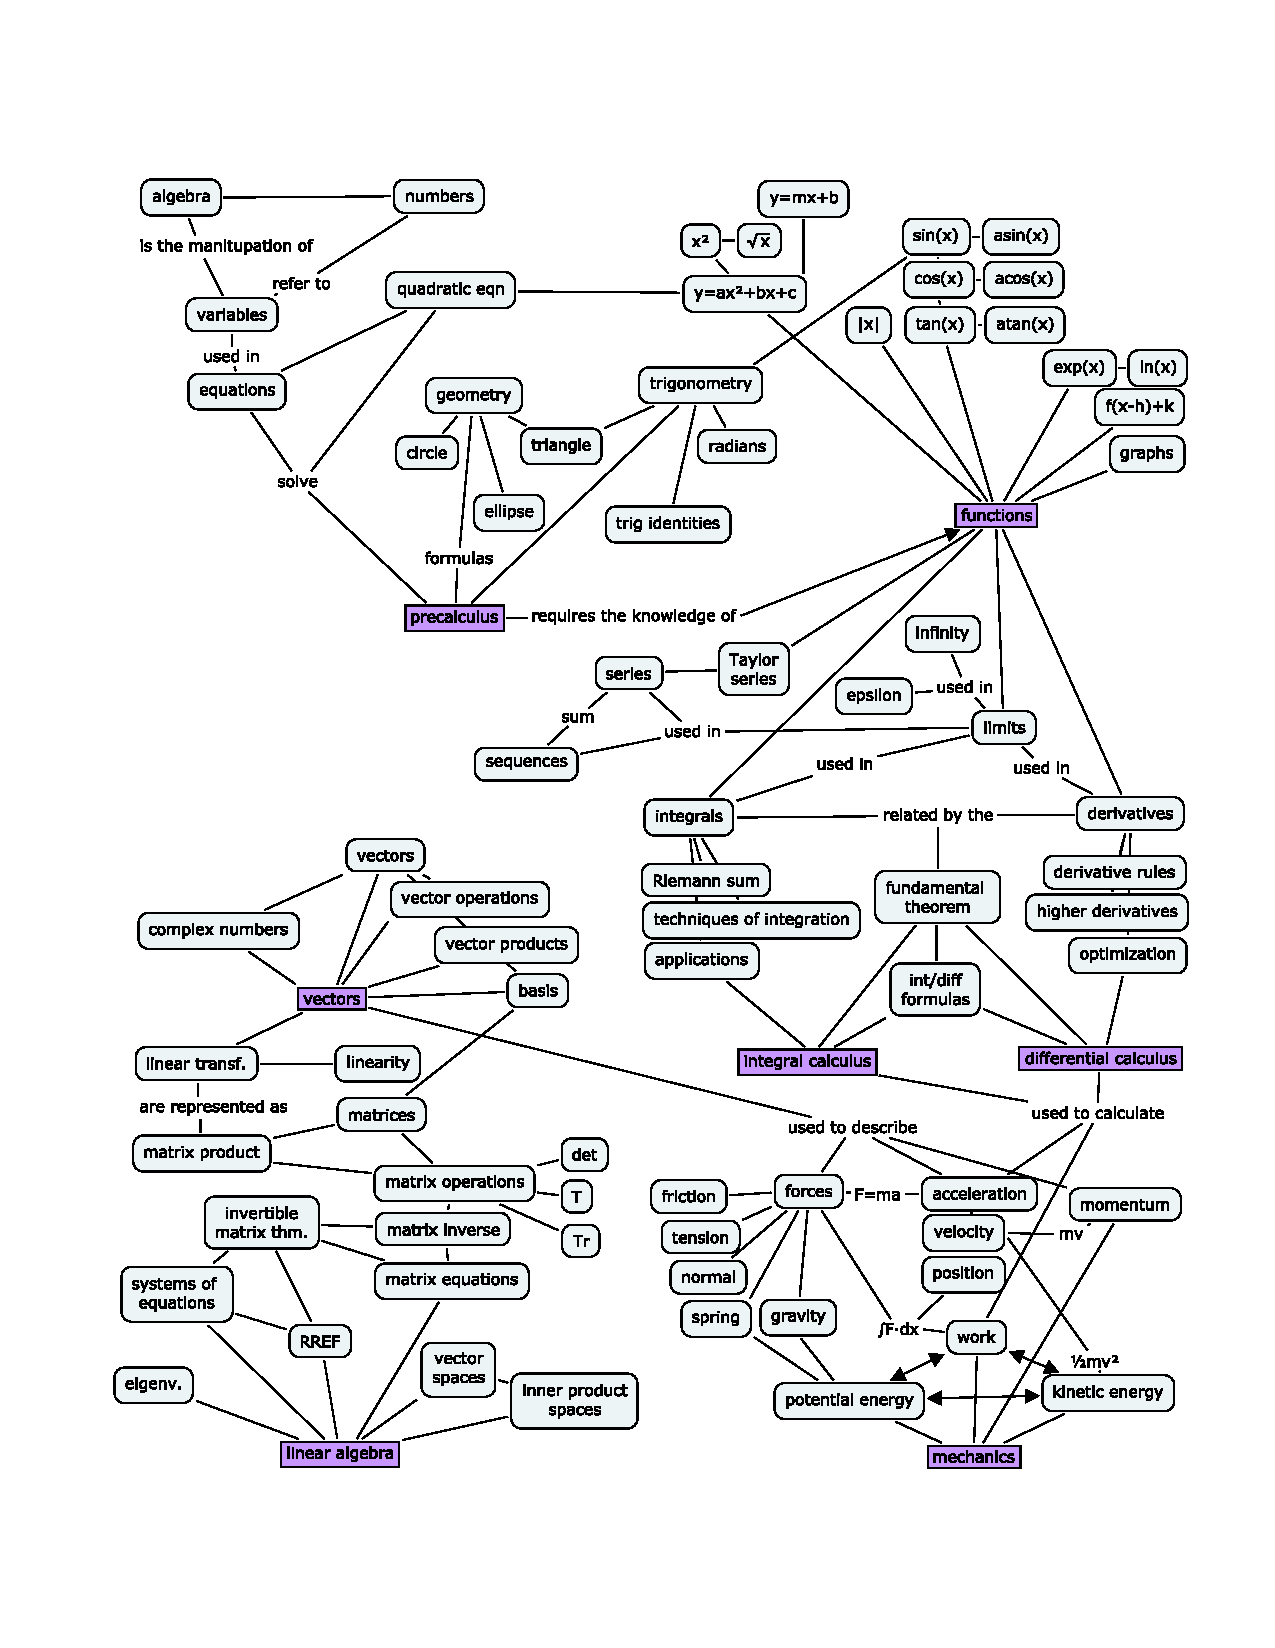
\includepdf{concept_map_last_page.pdf}
    
\end{document}
